\documentclass[aspectratio=169]{beamer}

% ---------- THEME & LOOK ----------
\usetheme{Madrid}
\usecolortheme{seahorse}
\usefonttheme{professionalfonts}
\setbeamertemplate{navigation symbols}{}
\setbeamercovered{transparent}
\setbeamertemplate{itemize items}[circle]
\setbeamertemplate{enumerate items}[default]
\setlength{\parskip}{0.25em}

% ---------- COLORS ----------
\usepackage{xcolor}
\definecolor{accent}{RGB}{0,92,184}
\definecolor{soft}{RGB}{233,244,255}
\setbeamercolor{structure}{fg=accent}
\setbeamercolor{title}{fg=white,bg=accent}
\setbeamercolor{frametitle}{fg=accent}
\setbeamercolor{block title}{bg=accent!10,fg=accent}
\setbeamercolor{block body}{bg=soft}

% ---------- PACKAGES ----------
\usepackage{booktabs}
\usepackage{amsmath, amssymb}
\usepackage{array}
\usepackage{graphicx}
\usepackage{hyperref}
\hypersetup{colorlinks=true,linkcolor=accent,urlcolor=accent}

% ---------- PLACEHOLDER BOX ----------
\newcommand{\placeholderbox}[2][0.82\linewidth]{%
  \begin{center}
    \fbox{\begin{minipage}[c][0.46\textheight][c]{#1}
      \centering \vspace{0.25em}
      \textbf{#2}\\[0.6em]
      \emph{Insert figure/table here later.}
    \end{minipage}}
  \end{center}
}

% ---------- TITLE ----------
\title{\textbf{Unemployment: Meaning, Measurement, and Canada's Experience}}
\subtitle{{\large ECON 300 - Labour Economics}}
\author{Muhebullah Karimzada}
\date{Winter 2026}

\begin{document}

% ============================================================
% TITLE
% ============================================================
\begin{frame}[plain]
  \titlepage
\end{frame}

% ============================================================
\section{Orientation}
% ============================================================

\begin{frame}{Learning Objectives}
\transfade
\begin{itemize}
  \item Explain how unemployment and the unemployment rate are defined and measured.
  \item Discuss controversies in measurement and alternatives.
  \item Summarize Canada's unemployment experience and cross-country comparisons.
  \item Define labour force participation and employment rates and explain why they matter.
  \item Define incidence and duration of unemployment and explain how they determine the unemployment rate.
  \item Describe the dynamic nature of the Canadian labour market and its implications.
\end{itemize}


\end{frame}

\begin{frame}{Main Questions}
\transfade
\begin{itemize}
  \item How is the unemployment rate measured? Who counts as unemployed?
  \item How does Canada compare internationally?
  \item How do incidence and duration contribute to the unemployment rate?
  \item How long is a typical Canadian unemployed, and how does this vary by group?
  \item Does the unemployment rate accurately reflect labour market hardship?
\end{itemize}

\begin{exampleblock}{Real Example}
Two countries can both have a 6\% unemployment rate, but one may have many short jobless spells while the other has fewer but much longer spells. The policy implications are very different.
\end{exampleblock}
\end{frame}

% ============================================================
\section{Measurement Basics}
% ============================================================

\begin{frame}{Measuring Unemployment (LFS Basics)}
\transfade
\begin{itemize}
  \item \textbf{Unemployed:} not currently employed and actively searching for work at prevailing wages and conditions.
  \item \textbf{Employed:} did any work for pay.
  \item \textbf{Labour force = employed + unemployed.}
  \item \textbf{Unemployment rate = unemployed \(\div\) labour force.}
\end{itemize}

\begin{block}{Definition}
The \textbf{Labour Force Survey (LFS)} is Statistics Canada's main monthly survey used to measure employment and unemployment.
\end{block}

\begin{block}{Interpretation}
A person is not counted as unemployed unless they are actively searching. Someone without a job who has stopped searching is not in the labour force under the standard definition.
\end{block}
\end{frame}

\begin{frame}{Why Definitions Matter}
\transfade
\begin{itemize}
  \item The unemployment rate depends critically on who is classified as:
  \begin{itemize}
    \item employed,
    \item unemployed,
    \item not in the labour force.
  \end{itemize}
  \item Classification rules create comparability over time and across countries.
  \item But these rules can hide some forms of labour market hardship.
\end{itemize}

\begin{exampleblock}{Real Example}
A university student working one paid hour in the survey reference week is counted as employed, even if they want a full-time job and cannot find one.
\end{exampleblock}
\end{frame}

% ============================================================
\section{Canadian Experience}
% ============================================================

\begin{frame}{Canadian Experience: A Brief Narrative}
\transfade
\begin{itemize}
  \item 1929: Great Depression surge to about 20\% unemployment.
  \item WWII: unemployment fell sharply.
  \item Recessions in 1957--58, 1974--75, and 1981--82 caused major increases.
  \item Early 2000s recovery lowered unemployment to 6.0\% by 2006.
  \item 2008--09 crisis raised it to 8.3\%.
  \item Unemployment gradually declined after 2009.
\end{itemize}

\begin{block}{Interpretation}
Canadian unemployment is strongly cyclical: it rises sharply in recessions and falls during expansions.
\end{block}
\end{frame}

\begin{frame}{Why Does Unemployment Change Over Time?}
\transfade
\begin{itemize}
  \item Aggregate demand shocks reduce firms' need for labour.
  \item Technological and structural changes alter demand across industries.
  \item Policy, demographics, and labour force growth also matter.
\end{itemize}

\begin{exampleblock}{Real Example}
During the 2008--09 financial crisis, output fell internationally. Canadian unemployment rose, but the increase was smaller than in some other advanced economies because Canada's financial sector was less severely damaged.
\end{exampleblock}
\end{frame}

\begin{frame}{Figure 16.1: A Century of Unemployment in Canada}
\centering
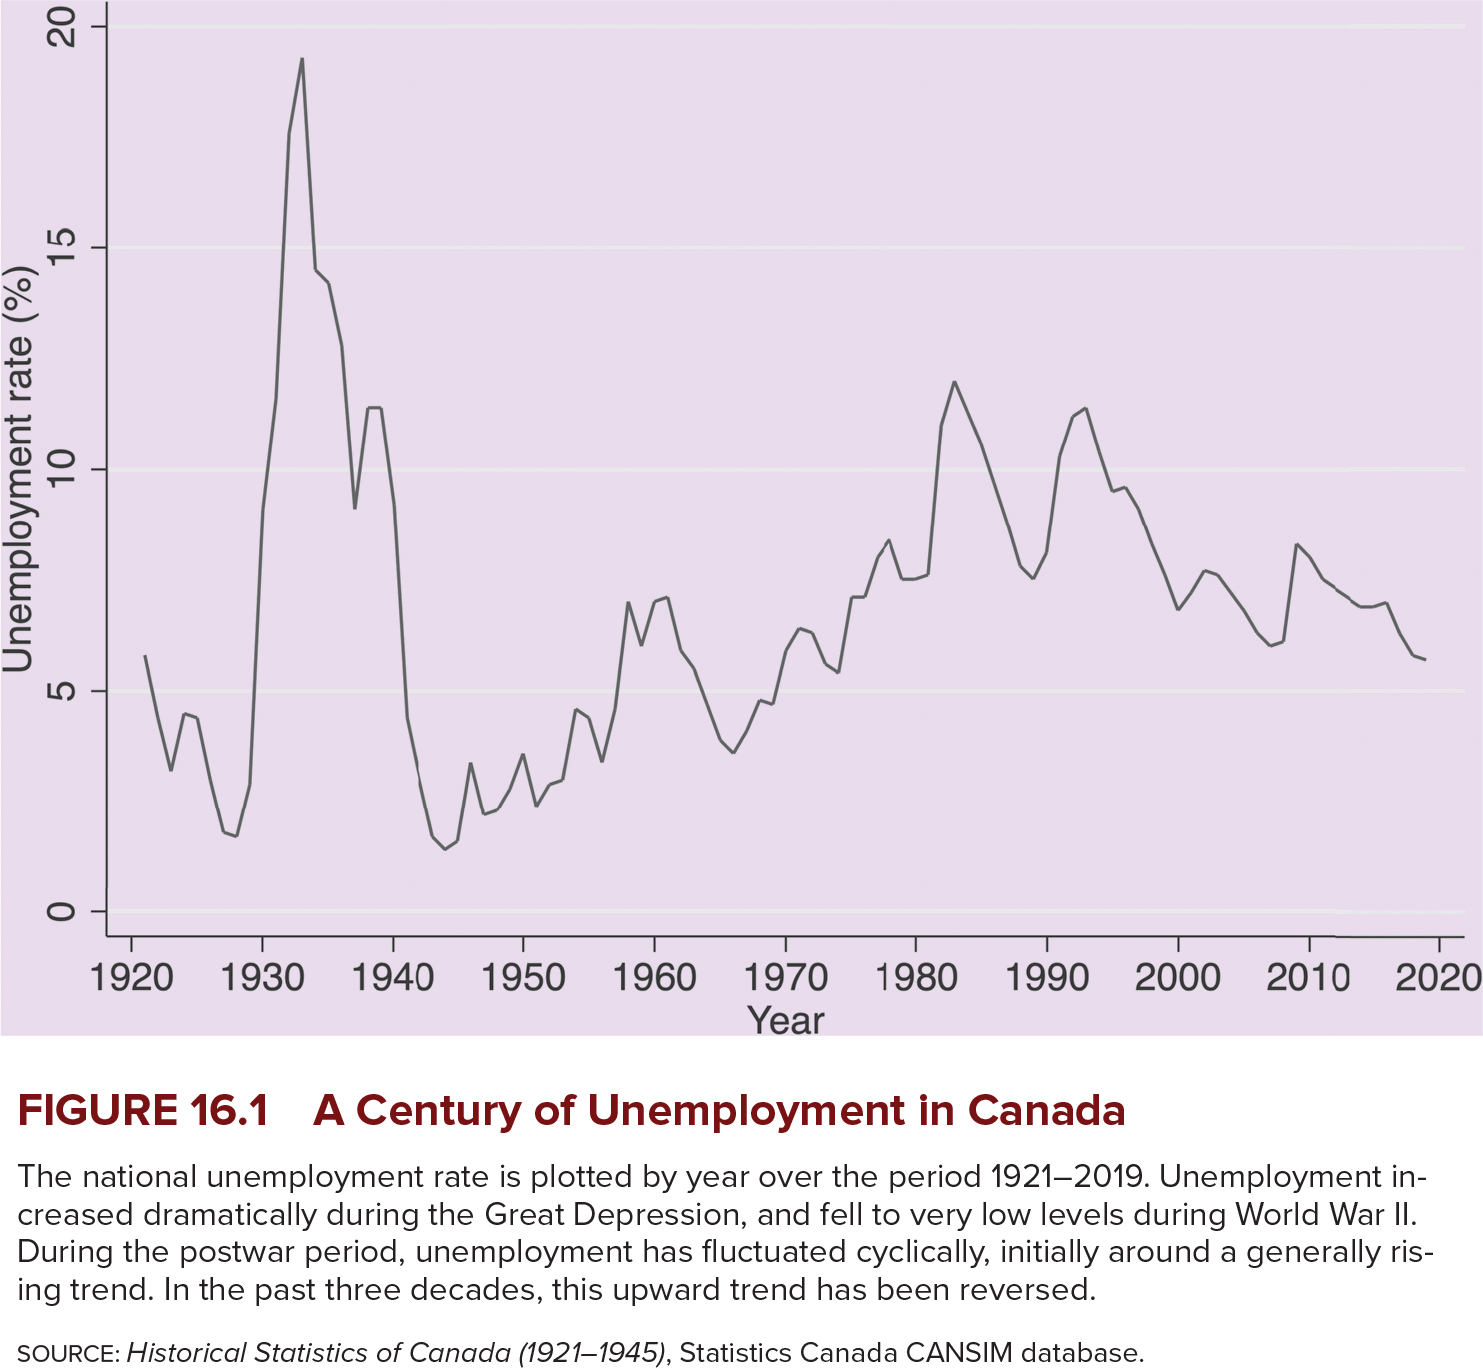
\includegraphics[width=0.68\linewidth]{ben54842_1601}
\end{frame}

\begin{frame}{Reading Figure 16.1}
\transfade
\begin{itemize}
  \item The figure shows large spikes during the Great Depression and major recessions.
  \item The long-run pattern suggests unemployment fluctuates with macroeconomic conditions rather than staying fixed.
  \item It also shows that today's ``normal'' unemployment rates are low relative to the worst historical episodes.
\end{itemize}

\begin{block}{Interpretation}
The unemployment rate is a macroeconomic indicator. It reflects the state of the whole economy, not just the experience of a single worker.
\end{block}
\end{frame}

% ============================================================
\section{Alternative Measures}
% ============================================================

\begin{frame}{Alternative Measures of Labour Force Activity}
\transfade
\begin{itemize}
  \item \textbf{Unemployment rate:} fraction of the labour force out of work and searching.
  \item \textbf{Employment rate:} fraction of the working-age population employed.
  \item \textbf{Labour force participation rate (LFPR):} fraction of the working-age population in the labour force.
\end{itemize}

\begin{block}{Definition}
The \textbf{working-age population} usually refers to people in the age range considered eligible and available for labour market activity.
\end{block}
\end{frame}

\begin{frame}{Why Use More Than One Indicator?}
\transfade
\begin{itemize}
  \item The unemployment rate can fall because more people find jobs.
  \item But it can also fall because discouraged workers leave the labour force.
  \item The employment rate and LFPR help distinguish these cases.
\end{itemize}

\begin{exampleblock}{Real Example}
If a recession causes many job seekers to stop looking, the unemployment rate may improve even though labour market conditions remain weak. The employment rate would reveal that weakness more clearly.
\end{exampleblock}
\end{frame}

\begin{frame}{Table 16.1: Labour Force Participation, Employment, and Unemployment, Canada, 1946--2019}
\centering
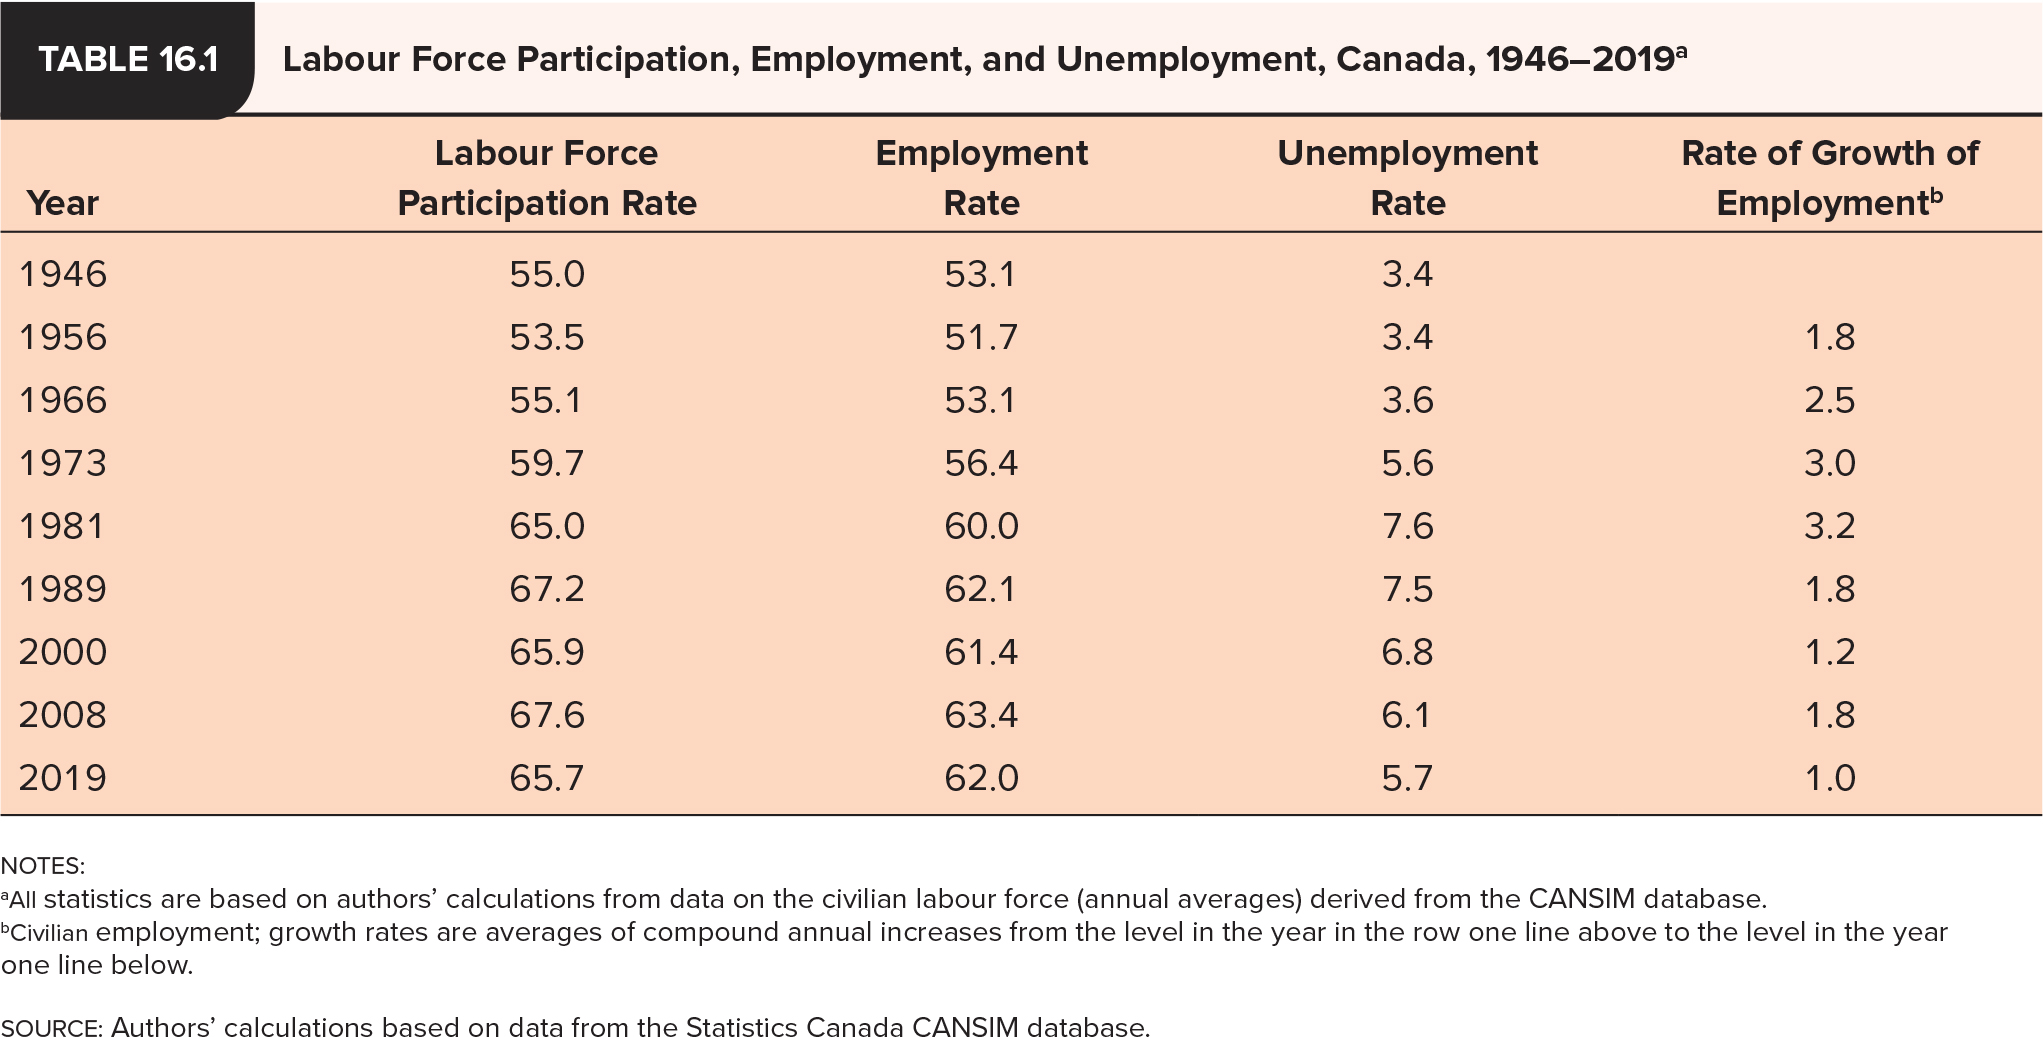
\includegraphics[width=0.95\linewidth]{ben54842_tb1601}
\end{frame}

\begin{frame}{How to Read Table 16.1}
\transfade
\begin{itemize}
  \item Participation and employment rates changed substantially over time.
  \item Rising female labour force participation was one major long-run trend.
  \item The unemployment rate alone does not summarize the whole labour market.
\end{itemize}

\begin{block}{Interpretation}
A country can have a moderate unemployment rate but low participation, which would indicate a weaker labour market than the unemployment rate alone suggests.
\end{block}
\end{frame}

% ============================================================
\section{International Differences}
% ============================================================

\begin{frame}{International Differences in Unemployment}
\transfade
\begin{itemize}
  \item In the 1950s, the U.S. had higher unemployment than Australia and Japan.
  \item The 1973 OPEC shock raised unemployment in several European countries.
  \item In the 1990s, France, Germany, and Italy experienced further increases.
  \item Since 2000, unemployment has generally been lower in many English-speaking countries.
  \item The 2008--09 crisis caused sharp increases across advanced economies.
\end{itemize}
\end{frame}

\begin{frame}{Why Do Countries Differ?}
\transfade
\begin{itemize}
  \item Business cycle conditions differ.
  \item Labour market institutions differ:
  \begin{itemize}
    \item employment protection,
    \item unemployment insurance,
    \item unionization,
    \item wage-setting systems.
  \end{itemize}
  \item Demographics and industrial structure also matter.
\end{itemize}

\begin{exampleblock}{Real Example}
Countries with stricter dismissal rules may experience lower job separation but longer unemployment duration if firms become more cautious about hiring.
\end{exampleblock}
\end{frame}

\begin{frame}{Figure 16.2: Unemployment Rates Across Selected Countries}
\centering
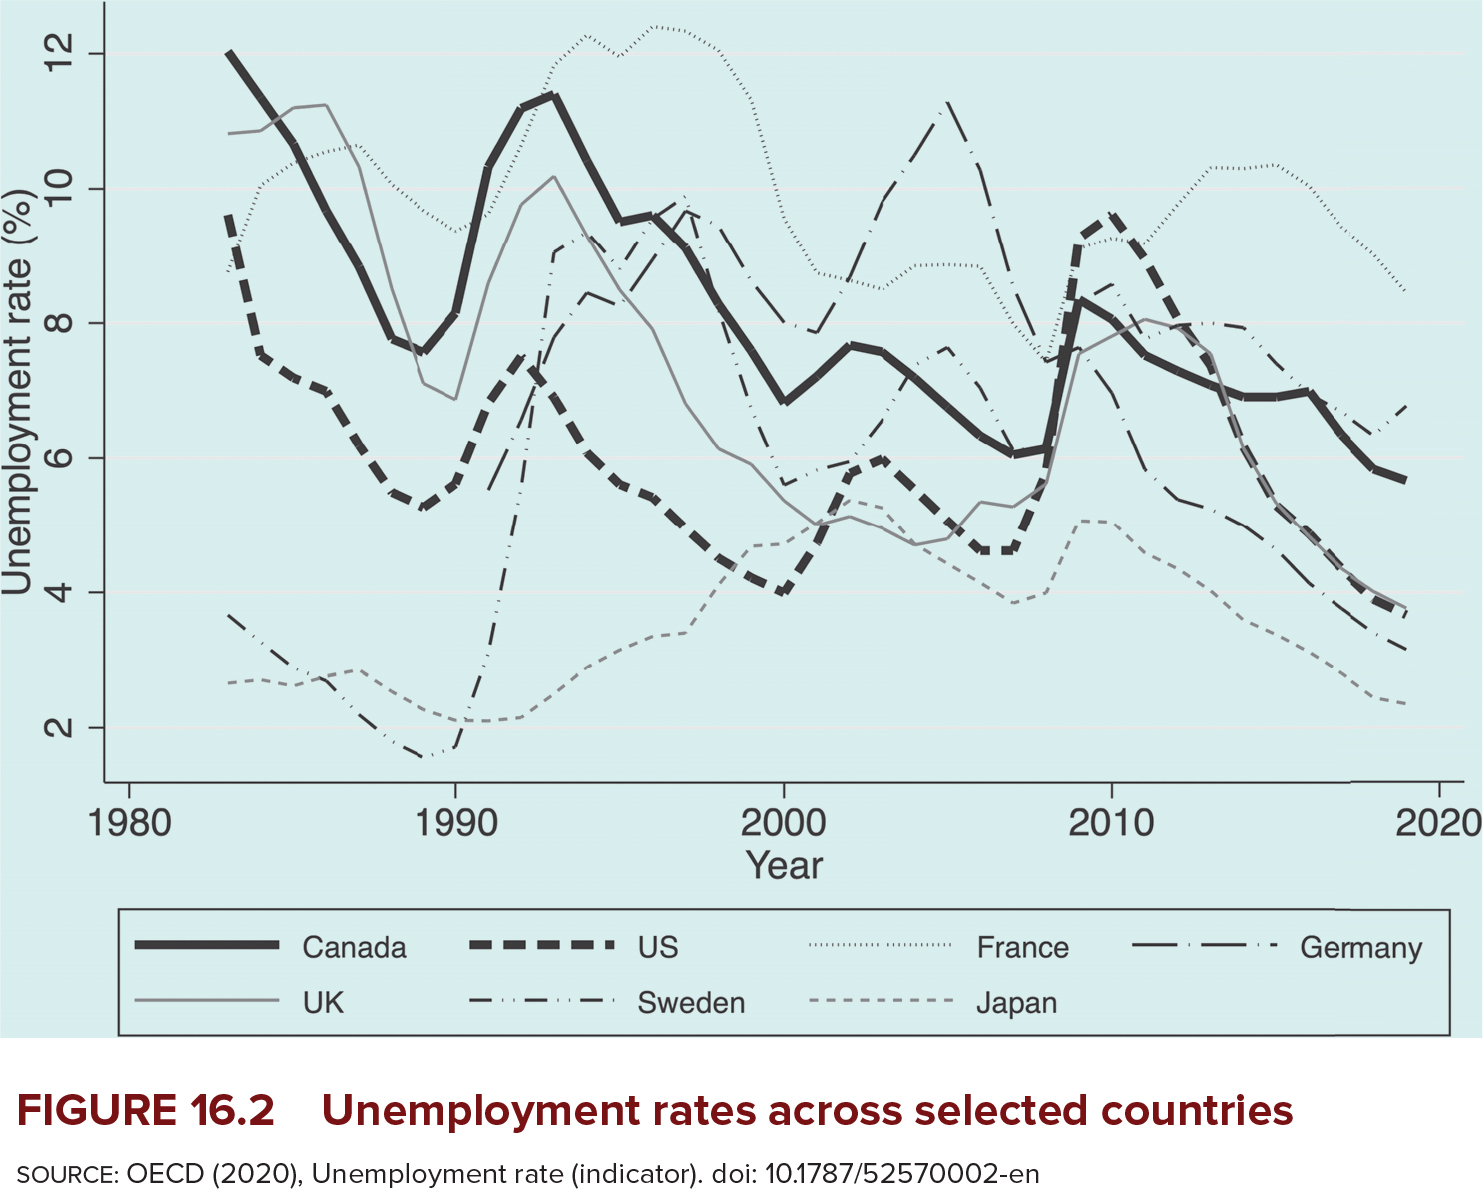
\includegraphics[width=0.68\linewidth]{ben54842_1602}
\end{frame}

\begin{frame}{Reading Figure 16.2}
\transfade
\begin{itemize}
  \item Canada moves broadly with other advanced economies, but not exactly one-for-one.
  \item Some countries show persistently lower unemployment, while others have more persistent high unemployment.
  \item The persistence of unemployment differs across countries.
\end{itemize}

\begin{block}{Interpretation}
Cross-country unemployment differences often reflect structural features, not only temporary macroeconomic shocks.
\end{block}
\end{frame}

% ============================================================
\section{Hidden Unemployment}
% ============================================================

\begin{frame}{Hidden Unemployment}
\transfade
\begin{itemize}
  \item Some people without work want jobs but are not counted as unemployed.
  \item \textbf{Discouraged workers} stop searching when jobs seem unavailable.
  \item Discouragement tends to rise in recessions.
\end{itemize}

\begin{block}{Definition}
\textbf{Hidden unemployment} refers to labour underutilization not captured by the official unemployment rate.
\end{block}
\end{frame}

\begin{frame}{Why Hidden Unemployment Matters}
\transfade
\begin{itemize}
  \item The official unemployment rate may understate labour market weakness.
  \item Discouraged workers may return to the labour force when conditions improve.
  \item Alternative indicators, such as broader underutilization measures, can be informative.
\end{itemize}

\begin{exampleblock}{Real Example}
After a major downturn, some people stop applying because they think no jobs are available. They disappear from the unemployment count, even though their hardship is real.
\end{exampleblock}
\end{frame}

% ============================================================
\section{Stocks and Flows}
% ============================================================

\begin{frame}{Labour Market Stocks and Flows}
\transfade
\begin{itemize}
  \item Workers move between:
  \begin{itemize}
    \item employment,
    \item unemployment,
    \item not in the labour force.
  \end{itemize}
  \item On average each month, many unemployed workers find jobs and many employed workers lose or leave jobs and start searching.
  \item The labour market is therefore highly dynamic.
\end{itemize}

\begin{block}{Definition}
A \textbf{stock} is the number of people in a category at a point in time. A \textbf{flow} is the movement between categories over a period.
\end{block}
\end{frame}

\begin{frame}{Why Flows Matter}
\transfade
\begin{itemize}
  \item The unemployment rate is a stock measure.
  \item But it is generated by flows into and out of unemployment.
  \item High unemployment can result from:
  \begin{itemize}
    \item many people becoming unemployed,
    \item few people exiting unemployment,
    \item or both.
  \end{itemize}
\end{itemize}

\begin{exampleblock}{Real Example}
In a deep recession, job separations rise and job-finding slows, so both inflows and duration worsen.
\end{exampleblock}
\end{frame}

\begin{frame}{Figure 16.3: Labour Market Stocks and Flows, 1976--1991}
\centering
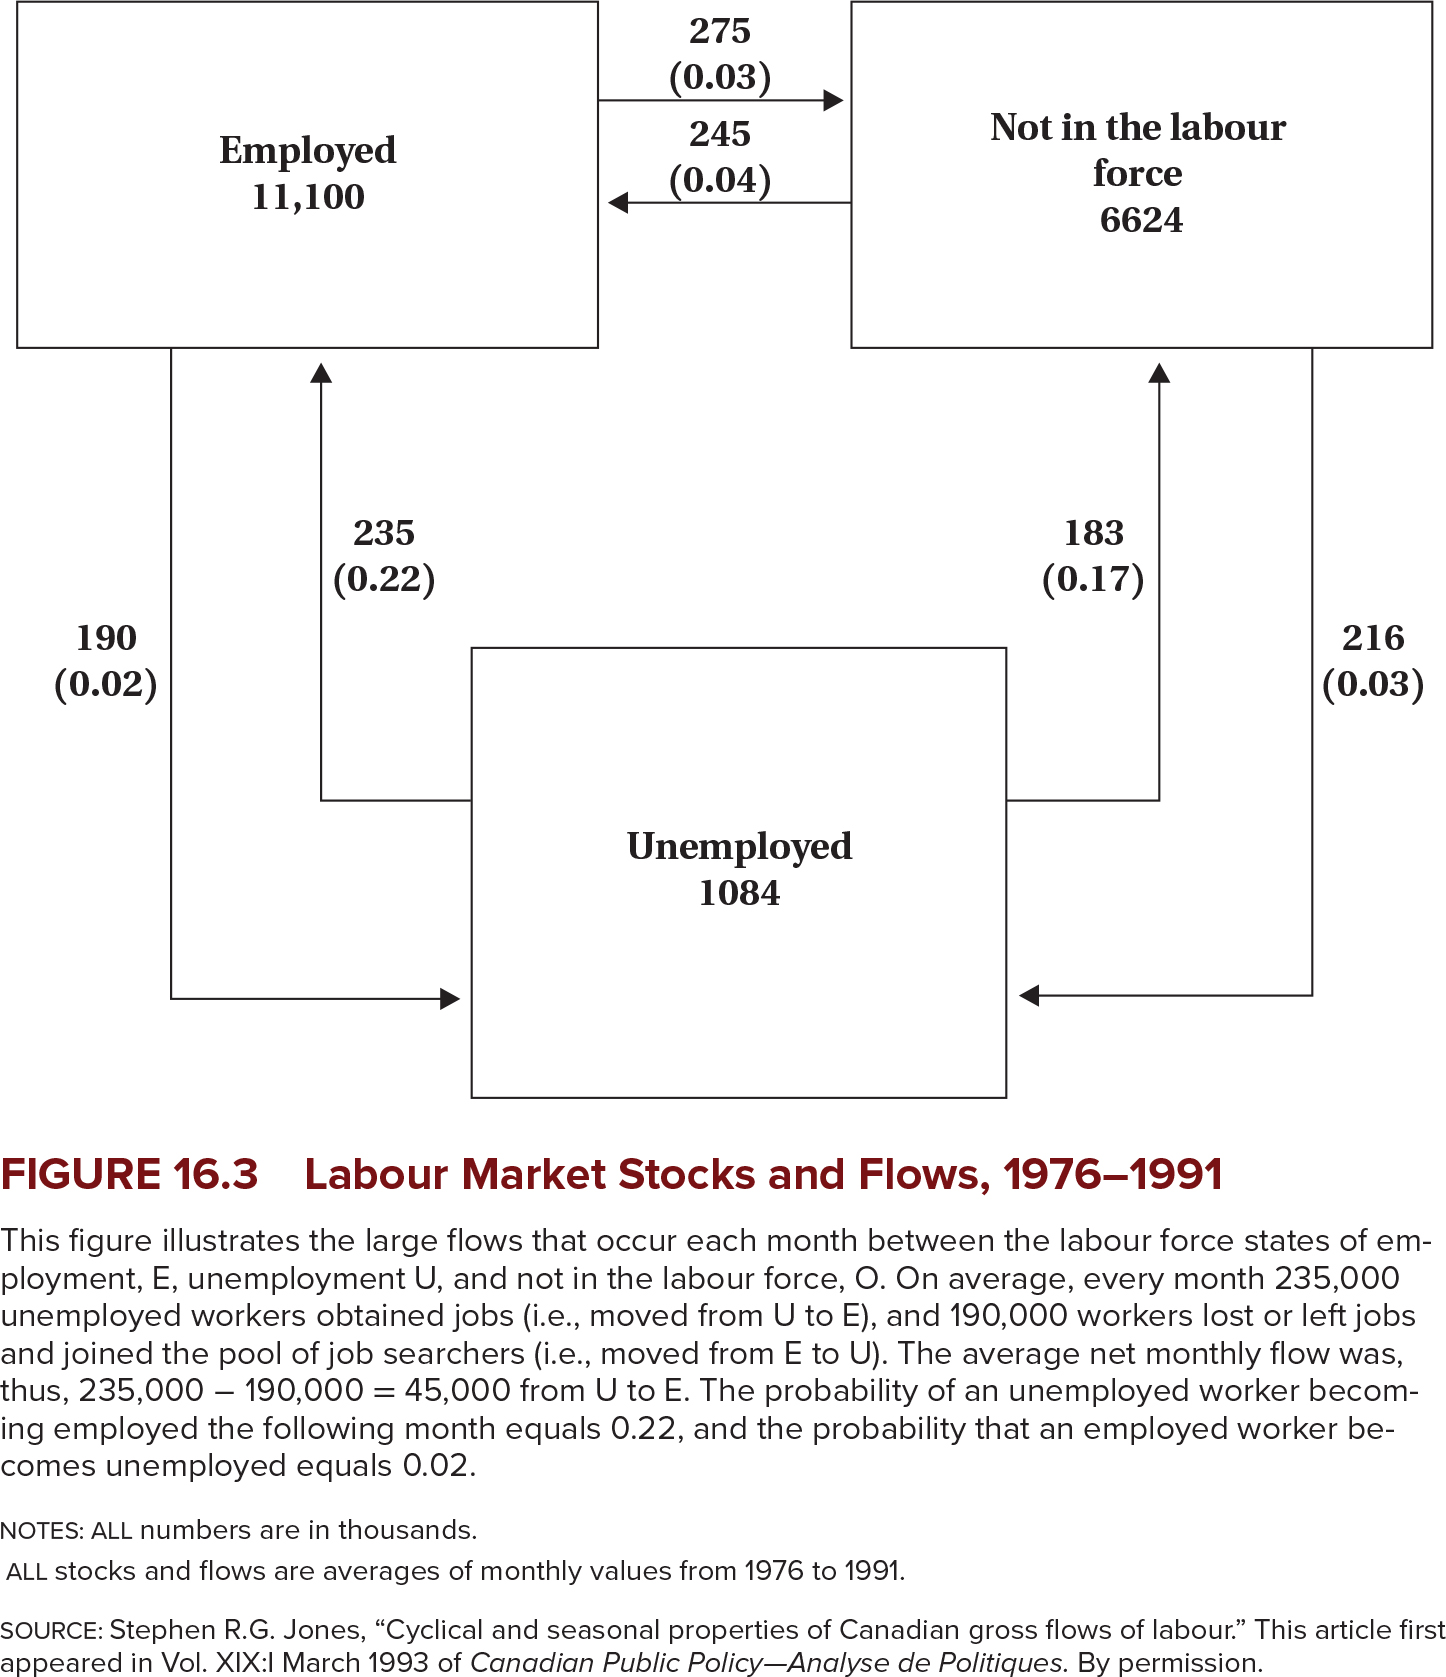
\includegraphics[width=0.65\linewidth]{ben54842_1603}
\end{frame}

\begin{frame}{Reading Figure 16.3}
\transfade
\begin{itemize}
  \item The boxes show the stock of employed, unemployed, and those not in the labour force.
  \item The arrows show average monthly flows among the three states.
  \item Even when the unemployment stock looks stable, many people are moving in and out.
\end{itemize}

\begin{block}{Interpretation}
Unemployment is not just a static condition. For many people it is a transition state between jobs, while for others it is a longer-term problem.
\end{block}
\end{frame}

\begin{frame}{Table 16.2: Decomposition of Unemployment by Reason, 2005--2019}
\centering
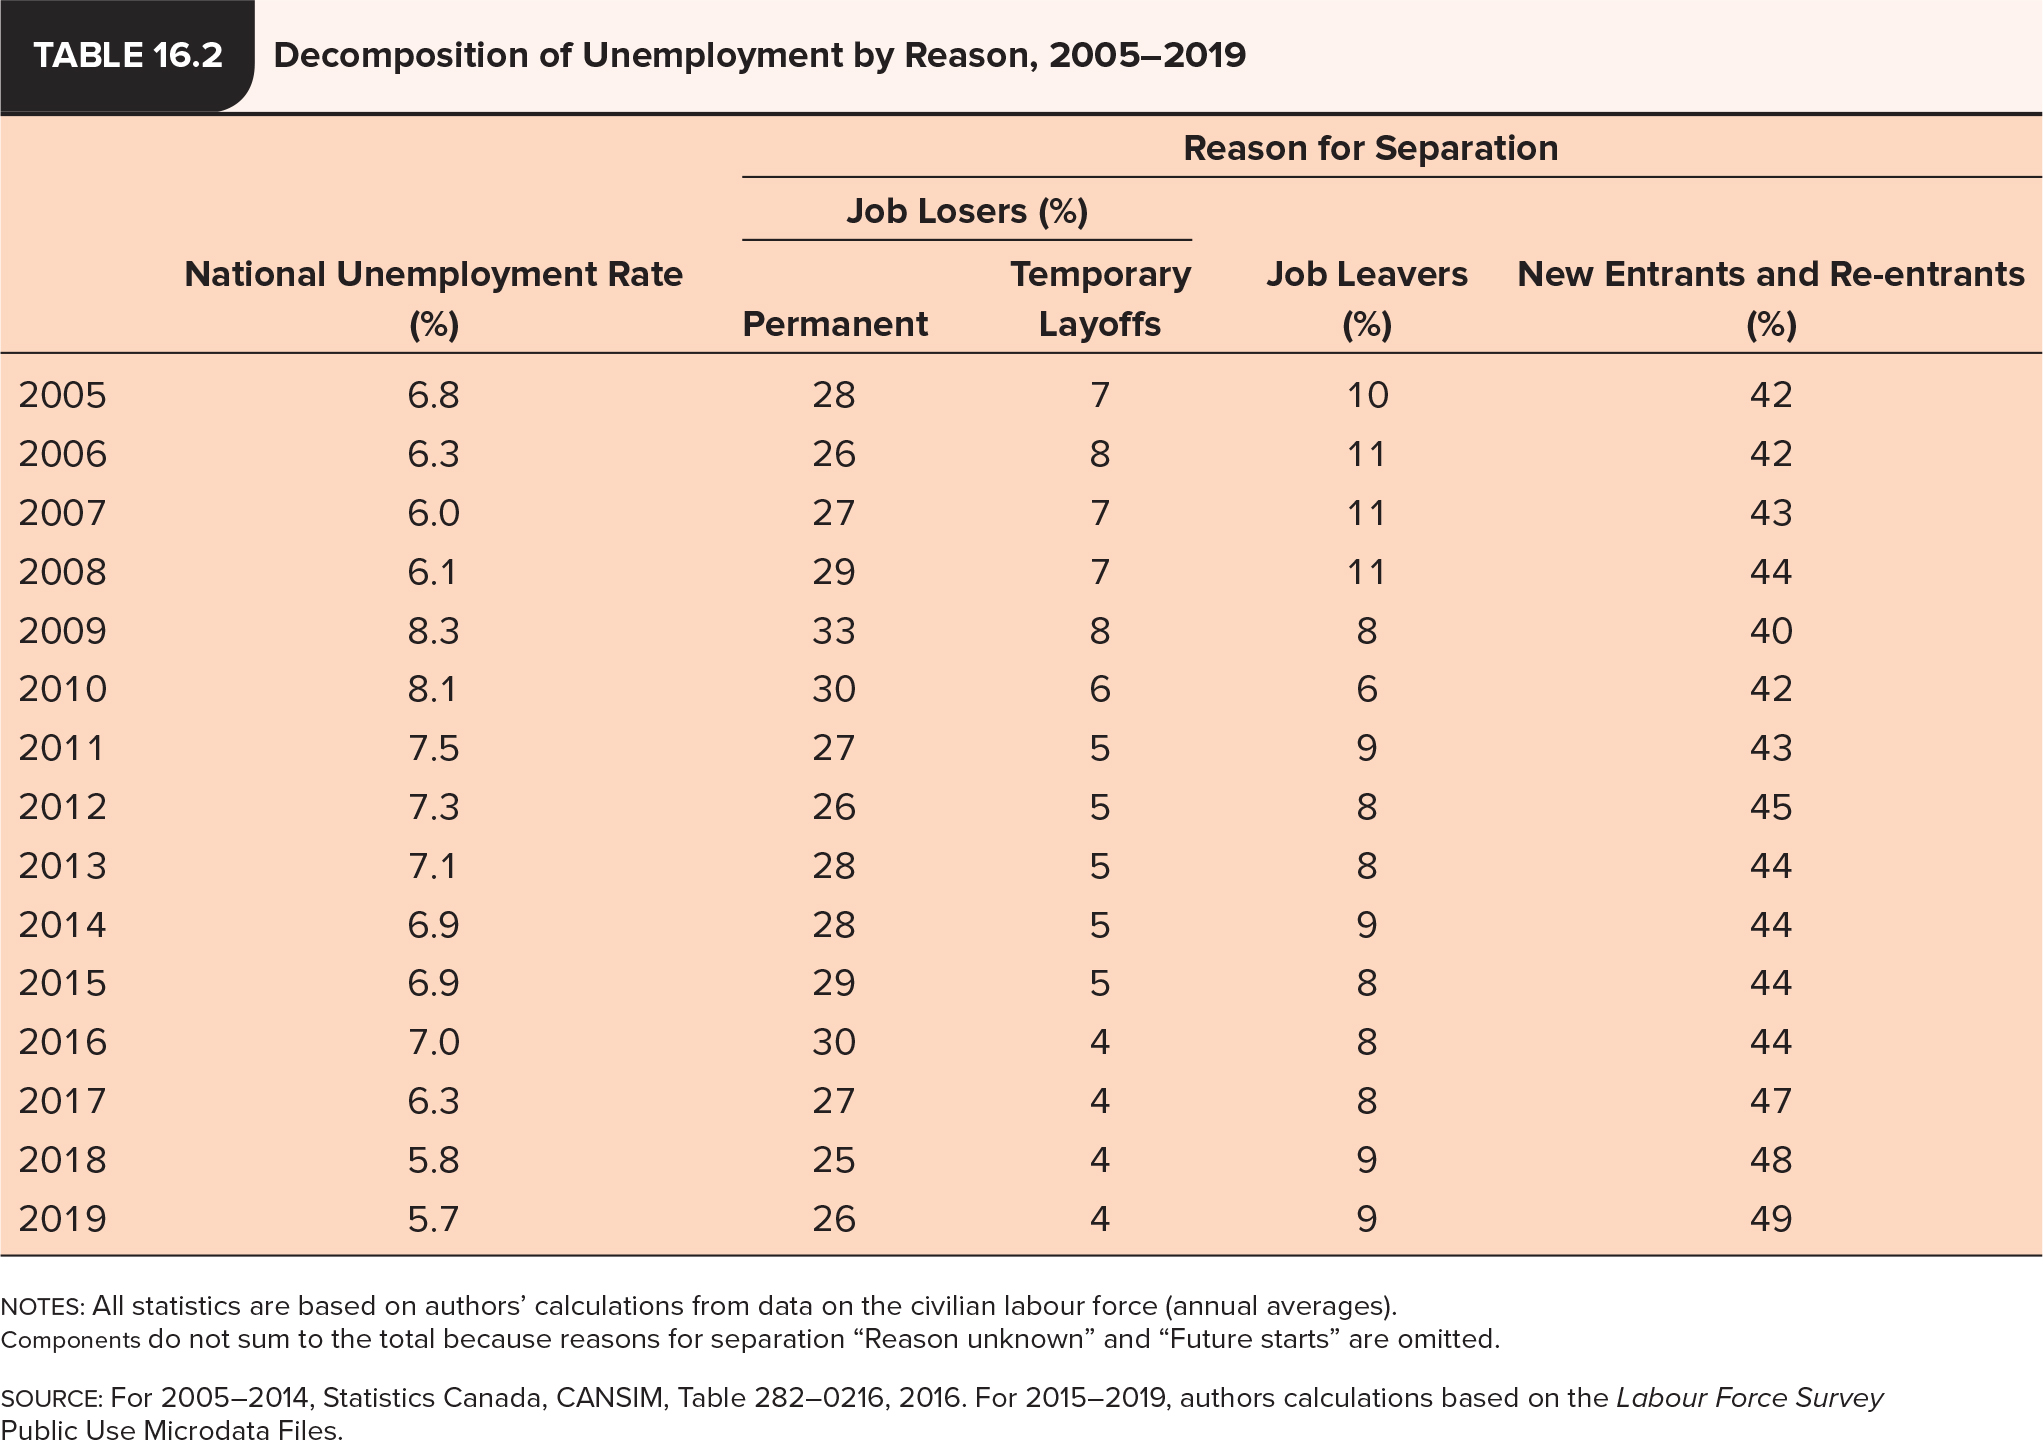
\includegraphics[width=0.735\linewidth]{ben54842_tb1602}
\end{frame}

\begin{frame}{How to Read Table 16.2}
\transfade
\begin{itemize}
  \item Unemployment arises for different reasons:
  \begin{itemize}
    \item permanent job loss,
    \item temporary layoff,
    \item job leaving,
    \item new entry or re-entry.
  \end{itemize}
  \item The composition changes over the cycle.
  \item During recessions, job loss tends to become more important.
\end{itemize}

\begin{block}{Interpretation}
The source of unemployment matters for policy. Job losers may need income support or retraining, while new entrants may need search assistance.
\end{block}
\end{frame}

% ============================================================
\section{Incidence and Duration}
% ============================================================

\begin{frame}{Incidence and Duration of Unemployment}
\transfade
\begin{itemize}
  \item \textbf{Incidence:} proportion of individuals who become unemployed in a period.
  \item \textbf{Duration:} length of time a person remains unemployed before exit.
  \item Both determine the unemployment rate:
  \[
  UR = \text{Incidence} \times \text{Duration}
  \]
\end{itemize}

\begin{block}{Definition}
This formula is a useful approximation showing that unemployment can be high because many people become unemployed, because unemployment lasts a long time, or both.
\end{block}
\end{frame}

\begin{frame}{Worked Example: Incidence vs. Duration}
\transfade
Two regions have the same unemployment rate, \(6\%\).

\begin{itemize}
  \item Region A: incidence \(= 3\%\), duration \(= 2\) months.
  \item Region B: incidence \(= 1.5\%\), duration \(= 4\) months.
\end{itemize}

\begin{block}{Interpretation}
The same unemployment rate can hide very different labour market realities:
\begin{itemize}
  \item Region A has frequent but short spells.
  \item Region B has fewer but longer spells.
\end{itemize}
\end{block}

\begin{exampleblock}{Policy Insight}
Region A may need better matching and job search tools. Region B may need stronger retraining or long-term income support.
\end{exampleblock}
\end{frame}

\begin{frame}{Table 16.3: Incidence and Duration by Age and Sex, Canada, 2019}
\centering
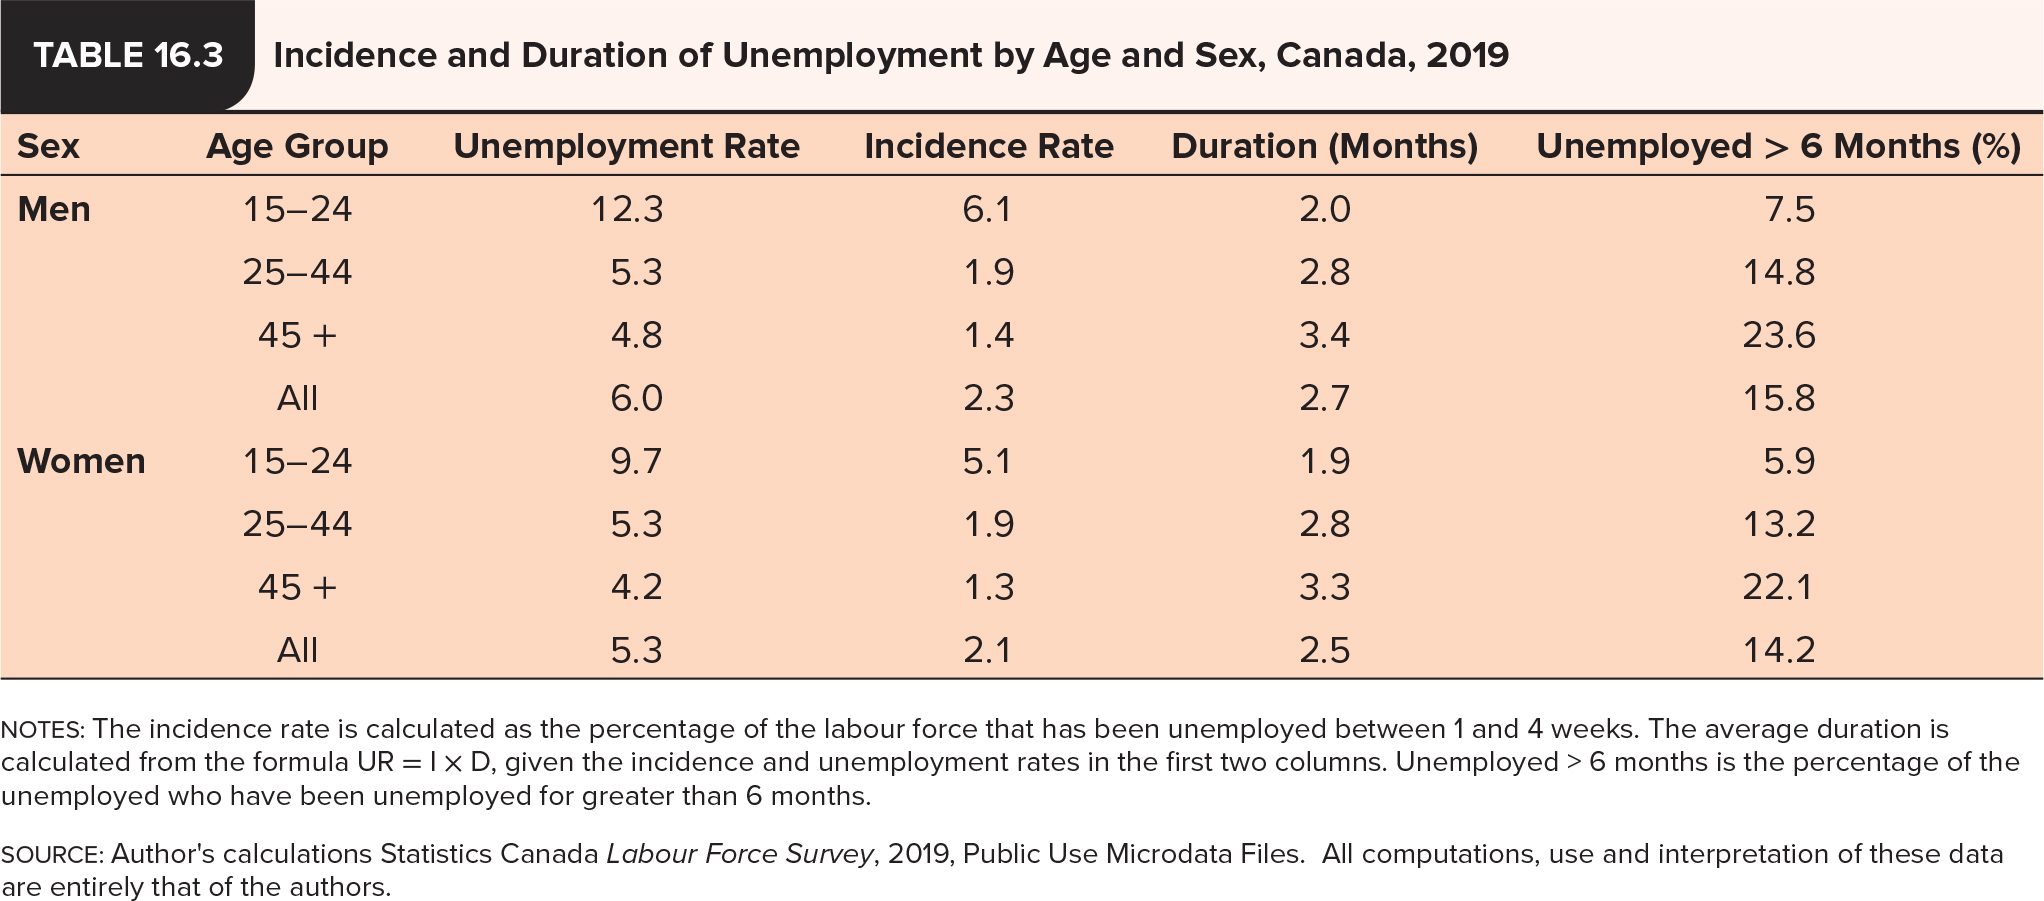
\includegraphics[width=0.95\linewidth]{ben54842_tb1603}
\end{frame}

\begin{frame}{Interpreting Table 16.3}
\transfade
\begin{itemize}
  \item Youth have the highest unemployment rates.
  \item But youth also have relatively short unemployment durations.
  \item Older workers have lower incidence but longer durations when unemployed.
\end{itemize}

\begin{block}{Interpretation}
Youth unemployment often reflects high turnover and entry into jobs, while older-worker unemployment is more likely to reflect long searches after displacement.
\end{block}

\begin{exampleblock}{Real Example}
A 19-year-old may move quickly between short jobs and short unemployment spells. A displaced 55-year-old may search much longer for a comparable job.
\end{exampleblock}
\end{frame}

% ============================================================
\section{Changing Perspectives}
% ============================================================

\begin{frame}{Changing Perspectives on Unemployment}
\transfade
\begin{itemize}
  \item The labour force is highly dynamic.
  \item Roughly half of inflows to unemployment are job losers.
  \item Even in years of above-normal unemployment, many spells remain relatively short.
  \item Younger groups have the highest unemployment rates because of high incidence, not necessarily because of very long durations.
\end{itemize}

\begin{block}{Interpretation}
Unemployment is not one uniform experience. Some workers experience brief transitions, while others face long-term exclusion from employment.
\end{block}
\end{frame}

\begin{frame}{Long-Term Unemployment in International Perspective}
\centering
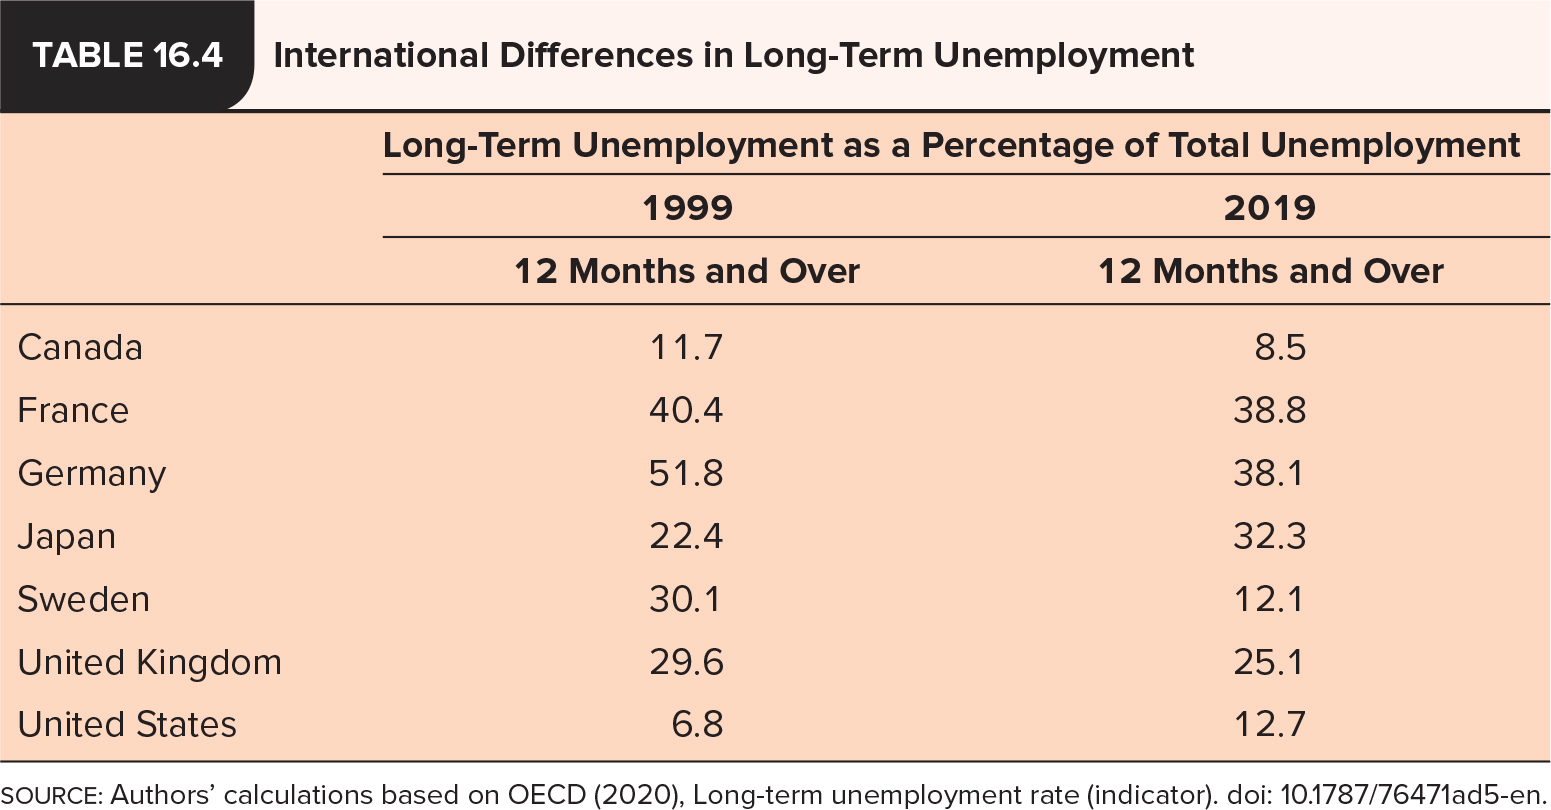
\includegraphics[width=0.92\linewidth]{ben54842_tb1604}
\end{frame}

\begin{frame}{Reading Table 16.4}
\transfade
\begin{itemize}
  \item Long-term unemployment is measured as the share of unemployment lasting 12 months or more.
  \item Countries differ substantially in the share of long-term unemployment.
  \item Canada's long-term unemployment share is relatively low compared with some European economies.
\end{itemize}

\begin{block}{Interpretation}
Two countries can have similar unemployment rates but very different long-term unemployment problems. Long-term unemployment is often more damaging because it weakens skills, earnings prospects, and attachment to the labour market.
\end{block}
\end{frame}

% ============================================================
\section{Unemployment Rate as Summary Statistic}
% ============================================================

\begin{frame}{Unemployment Rate as a Summary Statistic}
\transfade
\begin{itemize}
  \item The unemployment rate is widely used as an indicator of aggregate labour market conditions.
  \item It signals whether the labour market is tight or loose.
  \item It measures unused labour supply, but not all forms of labour market hardship.
\end{itemize}

\begin{block}{Interpretation}
A low unemployment rate usually indicates a stronger labour market, but it does not tell us everything about underemployment, hidden unemployment, or job quality.
\end{block}
\end{frame}

\begin{frame}{Strengths and Limitations of the Unemployment Rate}
\transfade
\begin{itemize}
  \item \textbf{Strengths:}
  \begin{itemize}
    \item simple,
    \item timely,
    \item widely understood,
    \item useful for tracking the business cycle.
  \end{itemize}
  \item \textbf{Limitations:}
  \begin{itemize}
    \item excludes discouraged workers,
    \item ignores underemployment,
    \item does not measure wage losses or job quality.
  \end{itemize}
\end{itemize}

\begin{exampleblock}{Real Example}
A part-time worker who wants full-time work counts as employed, even though their labour is underutilized.
\end{exampleblock}
\end{frame}

% ============================================================
\section{Summary}
% ============================================================

\begin{frame}{Summary}
\transfade
\begin{itemize}
  \item Unemployment is measured through the Labour Force Survey using clear rules for employment, unemployment, and labour force status.
  \item Canada's unemployment experience has varied greatly across the business cycle.
  \item Hidden unemployment and discouraged workers matter for interpretation.
  \item Stocks and flows show that the labour market is highly dynamic.
  \item The unemployment rate depends on both incidence and duration.
  \item International evidence on long-term unemployment highlights important structural differences.
\end{itemize}


\end{frame}

\begin{frame}
\centering
\Huge{\textbf{Thank You!}}
\end{frame}

\end{document}